%!TEX root = ../thesis.tex

\setcounter{secnumdepth}{4}

\chapter{Implementación}  %Title of the First Chapter
\label{capitulo4}

\graphicspath{{implementacion/Figs/Vector/}{implementacion/Figs/}}

Para el desarrollo de la aplicación se hizo uso del lenguaje \emph{Haskell} versión 8.0.2 y usando Cabal versión 1.24.2.0 como manejador de paquetes. Se escoge el lenguaje \emph{Haskell} sobre otros lenguajes funcionales por la consistencia que tiene este lenguaje a acatar de forma más estricta los conceptos asociados a la programación funcional y por ser un lenguaje compilado, lo que permite un mayor desempeño a tiempo de ejecución.

Dirigidos por la metodología de desarrollo por prototipos, se llevaron a cabo diversas iteraciones en las se expandió la funcionalidad del motor. Durante la primera iteración de trabajo se analizaron los métodos para graficar en \emph{Haskell} y se implementó el motor gráfico. En la segunda iteración se implementó el motor lógico y se establecieron los métodos con los cuales el programador puede implementar la lógica de su juego.  La tercera iteración se dedicó a la mejora del rendimiento del motor, añadiéndole la capacidad de correr los diferentes subsistemas en hilos de cómputo separados. La cuarta iteración, se añadió la capacidad para que el programador pueda correr funciones de E/S en forma asíncrona. En la quinta iteración se arreglaron desperfectos y se mejoró la interacción entre el motor y el programador según las experiencias obtenidas en los prototipos anteriores.

\section{Motor gráfico}

Este módulo debe contener las facilidades necesarias para el despliegue de gráficos en una ventana. La librería de despliegue gráfico seleccionada para el proyecto es OpenGL, que es una librería que interactúa con el GPU para brindar despliegue grafico acelerado por hardware. OpenGL tiene la ventaja de ser multiplataforma e independiente del sistema de ventanas y del sistema operativo en que corra la aplicación, permitiendo así a nuestra aplicación ser fácilmente portable entre diferentes dispositivos.

\subsection{Manejador de ventana}

La interfaz de OpenGL para \emph{Haskell} hace uso de la librería escrita en lenguaje c a través de la interfaz de funciones foráneas de \emph{Haskell}, haciendo necesario el uso de apuntadores e IO para poder interactuar con el contexto de OpenGL, siendo el objetivo de este módulo facilitar el despliegue gráfico, es importante hacer una librería que exponga una interfaz más funcional (de la misma forma en la que el monad IO oculta la naturaleza imperativa del mundo exterior) que sea más familiar a los usuarios de lenguajes funcionales y también que la librería provea de facilidades para cargar recursos multimedia al contexto de OpenGL así como controlar el proceso de despliegue gráfico.

El primer paso para usar OpenGL es la creación del contexto, para ello se ha elegido la librería GLUT, que es una librería de utilidades para aplicaciones que utilicen OpenGL, enfocándose primariamente en E/S a nivel de sistema operativo, operaciones como la creación y control de ventanas y entrada del teclado.

Trabajos realizados con GLUT se encuentran en el módulo \emph{EasyGLUT~\ref{EasyGLUT}}. La primera necesidad a la hora de usar GLUT está en definir callbacks para los diferentes eventos, entrada de mouse y teclado y cambios en el estado de la ventana. La motor gráfico provee funciones que inicializan una ventana GLUT (y consigo el contexto de OpenGL) y se definen diversos callbacks para el contexto de GLUT que procesan la entrada de la ventana y se acumula toda la entrada para ser procesada en el ciclo principal del programa.

Los callbacks definidos por el motor gráfico, permiten la detección de la entrada del usuario, que es almacenada en el tipo de dato \emph{MouseKey~\ref{MouseKey}}, que es una tupla que contiene un mapa del estado de las teclas y la posición del ratón. Usando esta información, el programador puede consultar en cualquier momento dado la entrada del jugador.

\begin{lstlisting}[label={MouseKey},frame=single,language=Haskell]
data KeyState = Down | Up | Pressed | Released deriving Show
data MouseState = FreeMouse GL.GLint GL.GLint | FixMouse GL.GLint GL.GLint
type MouseKey = (Map GLUT.Key KeyState,MouseState)
\end{lstlisting}

\subsubsection{GLUT como monad}

El motor gráfico también tiene la labor de manejar el ciclo principal de ejecución, y normalmente, al usar GLUT de forma convencional en \emph{Haskell}, este ciclo corre dentro del monad IO, permitiendo al usuario hacer cualquier cosa. Como la idea de un motor gráfico es que este se encargue de todos estos aspectos de E/S, se implementó el monad GLUT para sustituir al monad IO del ciclo principal del motor gráfico, y darle acceso al programador solo de las cosas que este pueda necesitar e impidiéndole alterar cosas que el motor gráfico controle.

Visto desde un punto de vista funcional, se puede considerar a GLUT como  un conjunto de cómputos que definen y controlan el estado de la ventana GLUT, así, estos cómputos pueden ser visto como un monad \cite{moggi1991notions} \cite{wiki:MonadsComputation} \cite{wiki:MonadsContainers}, que dentro de lenguajes funcionales facilitaría la interacción del usuario con la librería, ocultando apuntadores y demás detalles de comunicación con librería GLUT. De esta forma se introduce el monad GLUT que tiene las propiedades de poder ser consultado por eventos externos y entrada de dispositivos además de poder controlar una ventana de despliegue y un contexto de OpenGL.

\subsection{Carga de recursos}

Este módulo debe de proveer de herramientas para cargar recursos multimedia de formatos comunes. Esta sección tendrá un énfasis en imágenes y mallas poligonal que son los dos recursos multimedia con los cuales se puede hacer prototipos de juegos más rápidamente.

\subsubsection{Mallado poligonal}

El formato de archivos de mallado poligonal elegido para este proyecto es Wavefront .obj, que es un formato que guarda en forma simple información de geometría 3D en texto plano. Este es uno de los formatos más antiguos y es soportado por la gran mayoría de las herramientas de creación usadas por los artistas.

Ya que la información en un archivo Obj se guarda en texto plano, se crea un lexer y parser que puedan leer la información de un archivo. La información es guardada en el mismo formato en el tipo de dato Obj implementado en el módulo \emph{EasyGL.Obj~\ref{EasyGL.Obj}}.

\subsubsection{Imágenes}

Para la carga de imágenes se usa la librería JuicyPixels \cite{libreria:JuicyPixels} que soporta la lectura de imágenes en los formatos PNG, Bitmap, Jpeg, Radiance, Tiff y Gif. La carga de las imágenes se realiza en el módulo \emph{EasyGL.Material~\ref{EasyGL.Material}} al crear un material.

\subsection{Shaders}

El módulo \emph{EasyGL.Shader~\ref{EasyGL.Shader}} provee facilidades para cargar y compilar archivos de shaders a OpenGL. Todos los shaders compilados con esta librería poseerán atributos adicionales para recibir la posición del vértice, junto con su normal y coordenada de textura.

Este módulo ofrece funciones para cargar shaders de archivos y compilarlos. También implementa la función withShader que permite usar un shader en OpenGL de una manera funcional.

Adicionalmente, de la misma forma en que se realizó con GLUT,  se creó el monad Uniform que representa las acciones de cargar datos a los atributos de los shaders, que combinado con una clase Uniform, ayuda a garantizar que solo datos que puedan ser aceptados por el GPU sean cargados a este. Este monad premite la creación de la función withShaderSafe que permite usar un shader en forma segura ya que todo el pasaje de información al shader se hace por el monad Uniform.

\subsection{Materiales}

En el módulo \emph{EasyGL.Material~\ref{EasyGL.Material}} define el tipo de dato Material que contiene referencia a un shader ya compilado y a texturas que ya han sido cargadas a OpenGL. Este módulo solo ofrece la facilidad de cargar automáticamente texturas al shader contenido en el material.

\subsection{Cámara}

Se necesitan facilidades para el controlar los elementos a dibujar así como la perspectiva a usarse en los dibujos, este módulo debe ser capaz de utilizar los recursos cargados en otros módulos y producir imágenes en la ventana del juego. El módulo \emph{EasyGL.Camera~\ref{EasyGL.Camera}} ofrece una abstracción de cámara fácil de usar, que oculta las dificultades de configurar la visión en OpenGL así como la manipulación de matrices de transformación que ellos implican.

\subsection{Despliegue gráfico}

Para poder hacer uso de los mallados poligonales se debe primero cargar la información de los mismos al GPU. OpenGL hace uso de objetos conocidos como Vertex Array Object (VAO) y Vertex Buffer Object (VBO) como medios para almacenar información en el GPU y dibujar un objeto en pantalla de forma rápida y eficiente. Estos objetos pueden ser usados para cargar información de la posición de los vértices, la coordenada de las texturas y las normales del objeto, que es información que podemos obtener de los archivos Obj.

Ya que la información que se almacena en VAO's y en VBO's se ordena en forma diferente a la información almacenada en los archivos Obj, se implementó en el módulo \emph{EasyGL.IndexedModel~\ref{EasyGL.IndexedModel}} el tipo de dato IndexedModel, que almacena la información de un mallado (vertices, coordenadas de texturas y normales) en el orden y formato que se requiere para crear VAO's y VBO's. Uan gran ventaja que provee el dato IndexedModel, es que sirve como un intermediario para cargar información al GPU, y cualquier módulo que se agregue al proyecto para cargar algún formato de objeto poligonal al sistema, solo debe de implementar un método que convierta la información en un IndexedModel. Para cargar al GPU y dibujar en pantalla un IndexedModel, se usan las funciones implementadas en el modulo \emph{EasyGL.Entity~\ref{EasyGL.Entity}}.

Para cargar la información de los archivos Obj a OpenGL, se implementa el módulo \emph{EasyGL.Obj.Obj2IM~\ref{EasyGL.Obj.Obj2IM}}, que lee el archivo y transforma la información en un IndexedModel.

%\subsection{Extras}

%\subsubsection{Utils}
%\subsubsection{mem}

\section{Motor lógico}

Esta sección del programa se encargara de mantener y actualizar a los diferentes objetos del juego a medida que transcurre el tiempo. Este módulo debe de proveer al usuario las herramientas necesarias para implementar la lógica de su juego e inicializarlo al ser invocado. Para aprovechar las ventajas de la programación funcional la actualización de objetos debe de ejecutarse de una forma pura.

Permitir que el usuario implemente la lógica de su juego es de vital importancia para todo motor de juego, y como ya se mencionó en la \emph{sección~\ref{sec:MTlogica}}, los motores de juegos modernos emplean el patrón sistema entidad-componente, este patrón de diseño en su implementación depende en gran medida de la existencia de un estado mutable, la lógica creada por el usuario inevitablemente tiene que modificar componentes de una o más entidades para poder así generar cambios en el estado del juego. Sistemas implementados usando este patrón además requieren complejos sistemas para llevar a cabo la comunicación entre diversos subsistemas, y además, como muestra Jeff Andrews \cite{andrews2009designing}, la complejidad se hace mucho mayor cuando se quiere que estos sistemas corran de forma concurrente para hacer mejor use de procesadores modernos.

La implementación de un sistema que haga uso del patrón sistema entidad-componente en un lenguaje funcional como \emph{Haskell} es posible si se hace que todas las entidades se referencien con apuntadores y solo sean accesibles dentro del monad IO, semejante implementación podría dar los mismos resultados que en lenguajes imperativos, pero se incurriría en los mismos problemas sufridos en estos lenguajes además de no aprovechar ninguna de las ventajas que ofrece la programación funcional como las funciones puras.

La programación funcional reactiva es un paradigma de programación que nos permite sustituir al modelo sistema entidad-componente. Para este proyecto se ha decidido usar la librería \emph{Yampa}, que implementa \emph{FRP} y puede ser usado para mantener y actualizar una colección de entidades en forma pura.

\subsection{Tipos de datos}

Siguiendo el ejemplo de visto en “The Yampa Arcade” \cite{Courtney2003b}, podemos representar los objetos del juego como una SF que recibe como entrada el estado previo del juego y la entrada del jugador y retorna el nuevo estado del objeto así como la información necesaria para interactuar con los subsistemas del motor. Así un objeto tiene la forma:

\begin{lstlisting}[label={ObjDef1},frame=single,language=Haskell]
type Object = SF ObjInput ObjOutput
\end{lstlisting}

Esta abstracción nos permite distinguir los objetos de nuestro juego de otras SF. \emph{ObjInput} y \emph{ObjOutput} deben de ser definidos tomando en consideración que el usuario debe de poder usar su propio tipo de dato para representar el estado del juego y otro tipo de dato que represente los eventos que este quiera generar por su cuenta.

\begin{lstlisting}[label={ObjInputDef},frame=single,language=Haskell]
data ObjInput state eventType = ObjInput {
  oiEvents :: Event eventType,
  oiGameInput :: GameInput,
  oiPastFrame :: IL state
}
\end{lstlisting}

\emph{ObjInput} es definido como un tipo de dato que contiene la entrada del juego representada en el tipo GameInput, eventos que este objeto reciba y la colección de los objetos en el frame anterior del juego.

\begin{lstlisting}[label={ObjOutputDef},frame=single,language=Haskell]
data ObjOutput state eventType = ObjOutput {
  ooObjState :: !state,
  ooRenderer :: Maybe (ResourceIdentifier,Transform,Uniform ()),
  ooKillReq :: Event (),
  ooSpawnReq :: Event [Object state eventType],
  ooWorldReq :: [IOReq eventType],
  ooWorldSpawn :: [IO ()],
  ooUIReq :: [UIActions]
}
\end{lstlisting}

Cada registro del tipo \emph{ObjOutput} almacena:

\begin{itemize}
\item ooObjState: el estado de salida del objeto. Contiene la información relevante a la lógica del juego y es el único campo visible por otros objetos. Es estricto para garantizar que no existan fugas de memoria.
\item ooRenderer: este campo permite al objeto indicar al motor gráfico que dibujar. Si este campo contiene un Nothing entonces nada será dibujado en pantalla, de ser un Just, este contendrá una tupla con el id del mesh a usar, la posición en el espacio y los datos a enviar al shader.
\item ooKillReq: indica al sistema si se debe o no destruir el objeto.
\item ooSpawnReq: indica al sistema los nuevos objetos que se quiere crear.
\item ooWorldReq: hace al sistema iniciar una nueva operación de E/S cuyo resultado será de tipo \emph{eventType}. Este resultado será luego devuelto al objeto vía \emph{ObjInput} cuando esté disponible.
\item ooWorldSpawn: crea una nueva operación de E/S cuyo resultado no importa.
\item ooUIReq: permite interactuar con el manejador de ventana (GLUT en este caso).
\end{itemize}

Con la entrada y salida de nuestros objetos definidos, la nueva firma del tipo objeto pasa a ser:

\begin{lstlisting}[label={ObjDef2},frame=single,language=Haskell]
type Object outState eventType = SF
    (ObjInput outState eventType)
    (ObjOutput outState eventType)
\end{lstlisting}

Ahora que se ha definido el tipo de datos para los objetos del juego, es necesario poder crear una colección de estos objetos, esta colección requiere que cada objeto pueda ser identificado de manera única. En el módulo \emph{Val.Strict.IL~\ref{Val.Strict.IL}} se implementa el tipo de dato \emph{IL} (Identity List), \emph{IL} se define como:

\begin{lstlisting}[frame=single,language=Haskell]
type ILKey = Integer
data IL a = IL {
    ilNext :: ILKey,
    ilAssocs :: Map ILKey a
  }
\end{lstlisting}

El tipo \emph{IL} almacena los objetos en un mapa de la librería \emph{Data.Map}, que este posee muy buen tiempo para insertar, eliminar, consultar y recorrer, de usar un arreglo el tiempo para la inserción, la eliminación y la consulta serían mayores por requerir que los objetos sean identificables. Cada objeto es identificado con un \emph{ILKey} al momento de ser insertado.

Para hacer su uso lo más conveniente posible, el modulo \emph{Val.Strict.IL~\ref{Val.Strict.IL}} define múltiples funciones de consulta y modificación con \emph{IL}, además de incluir a \emph{IL} en las clases \emph{Functor}, \emph{Foldable}, \emph{Traversable} y \emph{NFData}.

\subsection{Escenas}
\label{sec:Escenas}

Para crear una escena de juego, se requiere primero una forma de actualizar la colección de objetos, para ellos se hace uso del dpSwitch de la librería \emph{Yampa}. Este suiche se caracteriza por manejar colecciones dinámicas de objetos, en el módulo \emph{Val.Strict.Scene~\ref{Val.Strict.Scene}} se hace uso de este suiche para crear la SF “sceneSF” que tiene la firma:

\begin{lstlisting}[frame=single,language=Haskell]
SF
  (GameInput, IL (ObjOutput s et), IL (Event et))
  (IL (ObjOutput s et))
\end{lstlisting}

La SF sceneSF recibe como entrada el estado de la ventana y entrada del usuario, el estado de los objetos en el frame anterior y eventos que deban ser enviados a objetos específicos, y retorna como resultado los objetos actualizados.

Con sceneSF es posible ahora implementar el ciclo principal del juego, el módulo \emph{Val.Strict.Scene \ref{Val.Strict.Scene}} implementa la función initScene, que dado la información de los recursos a usar, una SF que controle una cámara y una colección inicial de objetos, carga todos los recursos al sistema e inicia el ciclo principal.

La función initScene inicia la escena del juego creando tres hilos de cómputo encargados de tareas específicas, en la \emph{Figura~\ref{fig:ciclo_de_juego}} se puede apreciar el flujo de los datos entre los hilos. Cada hilo esta e
encargado de:

\begin{itemize}
\item Hilo 1, hilo lógico: Este hilo se caracteriza por actualizar la colección de objetos cada frame, este hilo inicia recibiendo la entrada del usuario del hilo 2 y el retorno de las funciones asíncronas generadas por los objetos manejados por el hilo 3. Con estos dos datos se actualizan los objetos en base al tiempo transcurrido y la salida de ellos es transmitida a los otros hilos.
\item Hilo 2, hilo de despliegue: Este hilo maneja el contexto de OpenGL y GLUT, inicia enviando la entrada del usuario al hilo 1 y recibe la salida de los objetos generados en el hilo 1. Con esta salida se puede generar el despliegue de gráficos.
\item Hilo 3, hilo de E/S: Este hilo existe para que los objetos del juego puedan ejecutar funciones de E/S de manera asíncrona. Este hilo mantiene una lista de todas las funciones asíncronas en corrida. Este hilo inicia evaluando la culminación de alguna función y enviando los resultados al hilo 1, luego recibe la salida del hilo 1 y corre cualquier nueva función asíncrona que los objetos soliciten.
\end{itemize}

\begin{figure}[!htbp!]
\centering
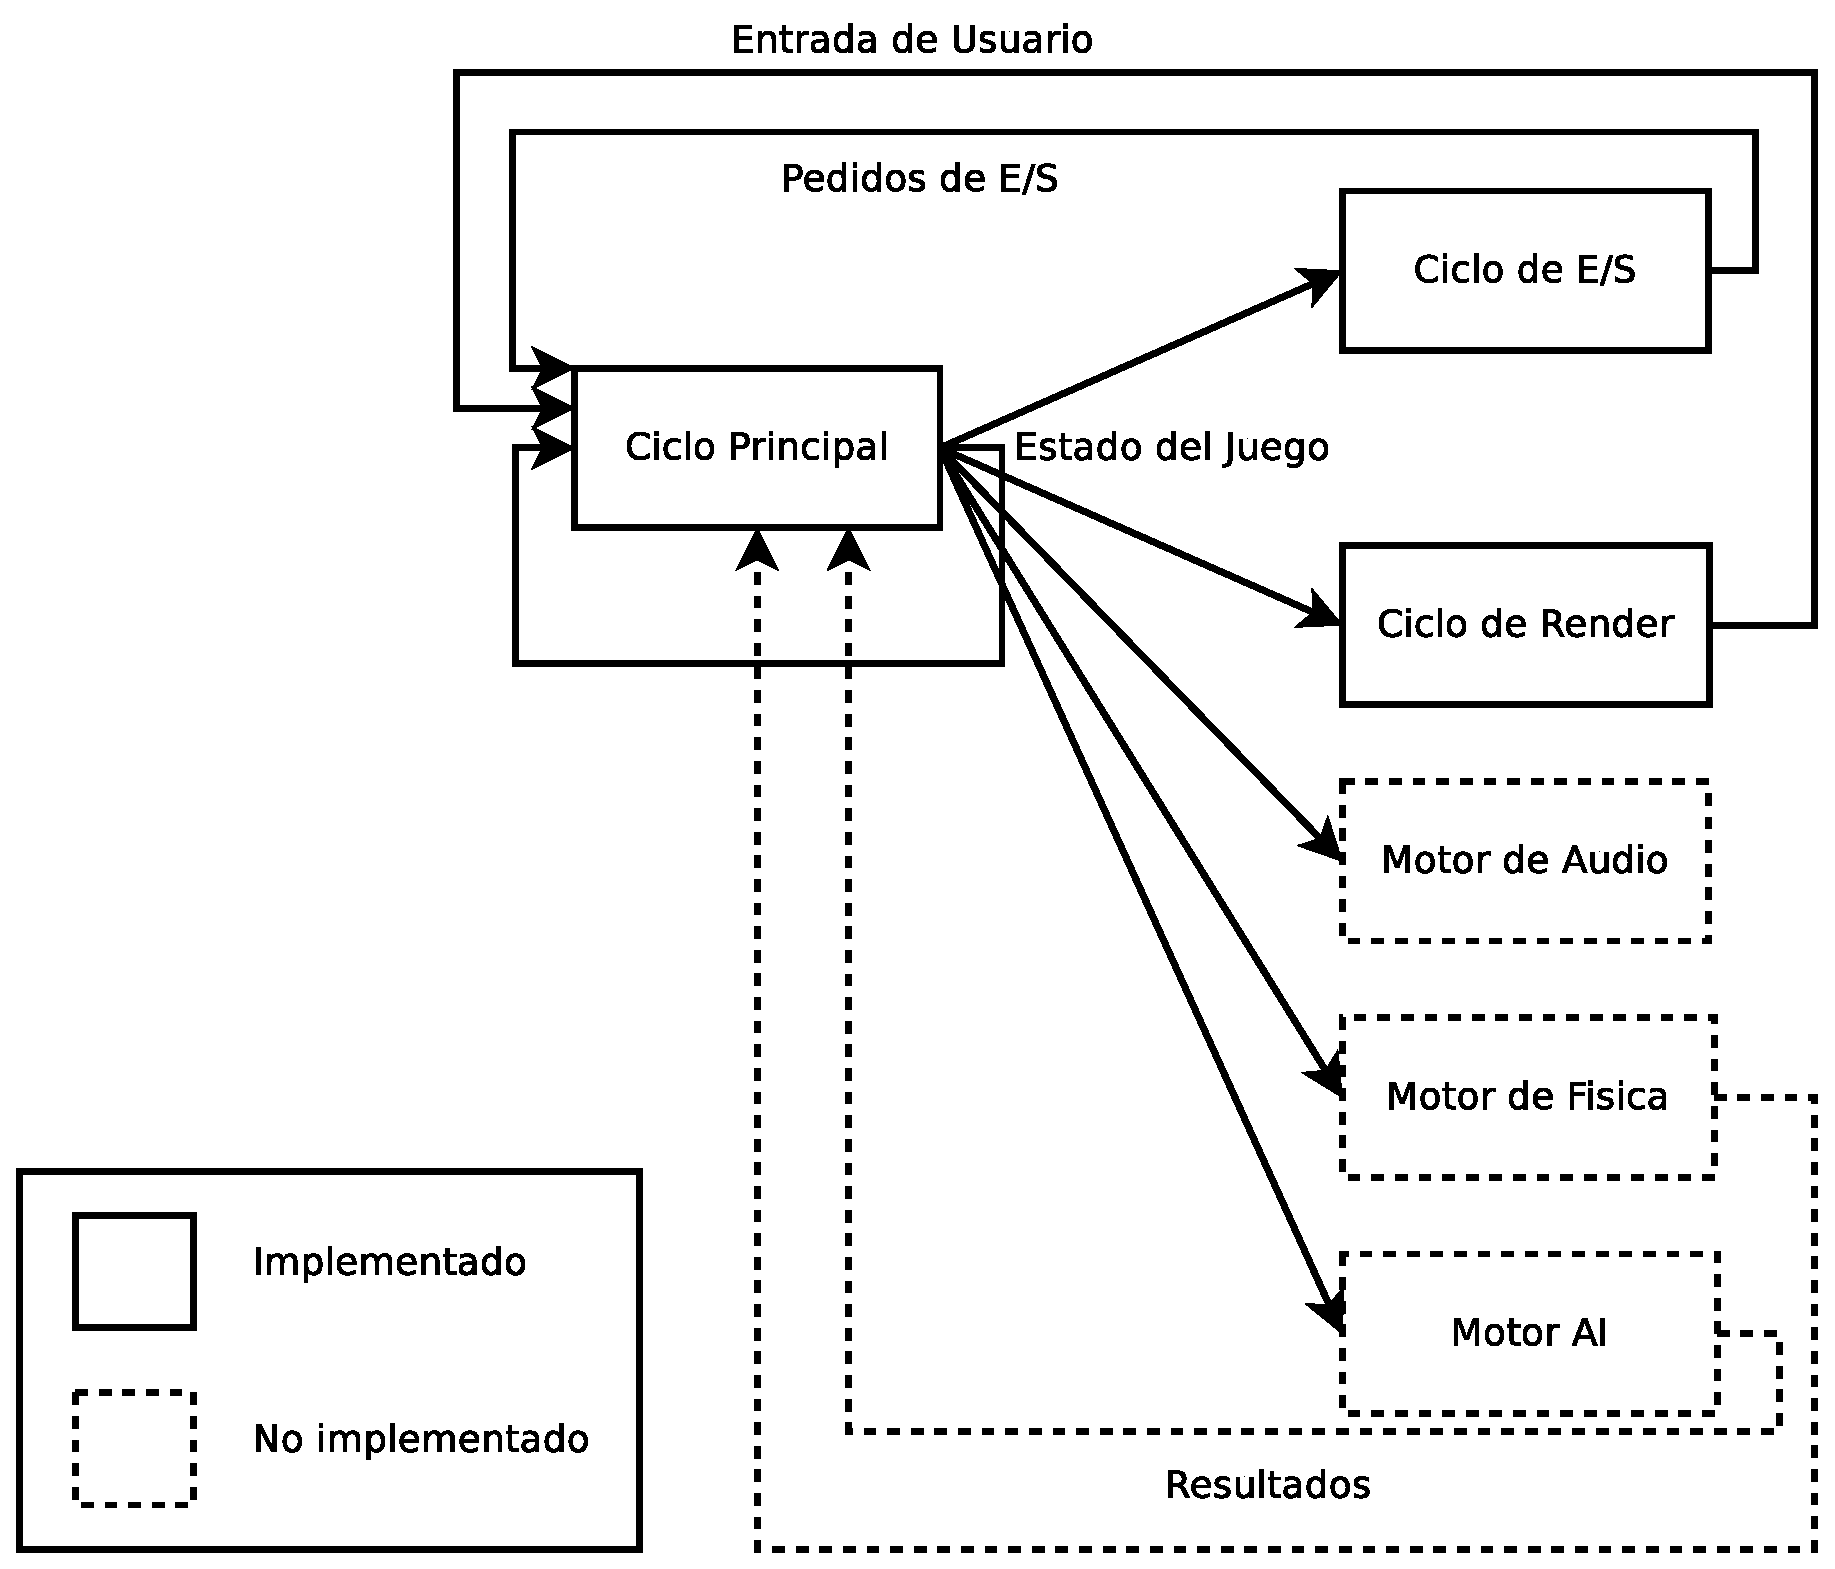
\includegraphics[width=1.0\textwidth]{ciclo_de_juego}
\caption[Ciclo de juego]{Esta figura muestra los diferentes hilos que corren en una escena de juego y a donde se envían los resultados de cada unos de ellos.}
\label{fig:ciclo_de_juego}
\end{figure}

Como cada hilo solo requiere de una referencia a los resultados de los objetos del juego para correr, que son valores inmutables y por lo tanto no pueden afectar a otros hilos, se puede añadir otros hilos nuevos con otro tipo de funcionalidad como sonido, networking, inteligencia artificial, entre otros, sin alterar el funcionamiento ya implementado y sin modificar la lógica actual.

La comunicación entre los diferentes hilos se logra con el uso de \emph{MVar}, que son apuntadores especiales de \emph{Haskell} que tienen la propiedad de funcionar como semáforos, haciendo que los hilos solo puedan enviar información a otros una vez estos estén listos para recibirla. El uso de estas \emph{MVar} causa, en la implementación actual, que todos los hilos se sincronicen al más lento.

El módulo \emph{Val.Strict.Scene~\ref{Val.Strict.Scene}} ademas aprovecha el hecho de que el tipo \emph{IL} implemente la clase \emph{Traversable}, con esta clase se puede usar la librería \emph{Control.Parallel.Strategies} de \emph{Haskell} para que el calculo de los diferentes objetos del juego se realice en forma concurrente manejado por el runtime environment de \emph{Haskell}, permitiendo que los cálculos realizados en el hilo lógico puedan realizare en más de un procesador. Para poder usar esta versión del hilo lógico, el usuario solo debe cambiar la llamada de la función initScene por la función initScenePar implementada en el mismo módulo.

\subsection{Utilidades}

Ya que \emph{FRP} es un concepto complicado (de aprender a usar), puede resultar ser una barrera para usar el motor de juego, por ello se ha creado en el módulo \emph{Val.Strict.Util~\ref{Val.Strict.Util}} la función makeSF que tiene la firma:

\begin{lstlisting}[frame=single,language=Haskell]
makeSF :: a
  -> (a -> ObjInput b c -> (a,ObjOutput b c))
  -> Object b c
\end{lstlisting}

Con la función makeSF el usuario puede crear un objeto de juego sin usar \emph{FRP} o la librería \emph{Yampa}. Esta función toma como primer argumento un estado inicial y de segundo una función que toma ese estado, una entrada de objeto y retorna el estado actualizado y una salida de objetos.

Sin embargo esta forma de crear objetos de juego carece de la capacidad de cambiar comportamiento a medida que corre el programa que posee \emph{FRP}, un objeto creado con esta función solo podrá tener el comportamiento de la función dada en el segundo argumento. La única manera de cambiar el comportamiento es creando un objeto nuevo y destruir el viejo.
